\section{Explaining Type Errors With Traces}
\label{sec:explaining}

A trace, on its own, is too detailed to be
a good explanation of the type error. One approach
is to use the witness input to step through the
program with a \emph{debugger} to observe how
the program evolves.
%
This route is problematic for two reasons.
%
First, existing debuggers and interpreters for
typed languages (\eg\ \ocaml) typically require
a type-correct program as input.
%
Second, we wish to have a quicker way to get
to the essence of the error, \eg\ by skipping
over irrelevant sub-computations, and focusing
on the important ones.

Next, we present a novel way to debug executions.
%
First, we develop a notion of a \emph{reduction graphs}
and extend our semantics with a form of \emph{tracing}
so that they incrementally collect the edges
in the graph (\S~\ref{sec:inter-semant}).
%
Next, we express a set of common \emph{interactive debugging}
steps as graph traversals (\S~\ref{sec:traversing-graph}), yielding
an novel interactive debugger that allows the user
to effectively visualize \emph{how} the program goes (wrong.)

% The trace takes the form of a \emph{reduction graph}, where the nodes
% are terms and the edges represent either the single-step
% $\hookrightarrow$ or a ``sub-term'' relation. For example, evaluating
% the expression @1 + 2 + 3@ would produce the graph in
% Figure~\ref{fig:simple-reduction}.
% %
% \begin{figure}[t]
%   \centering
%   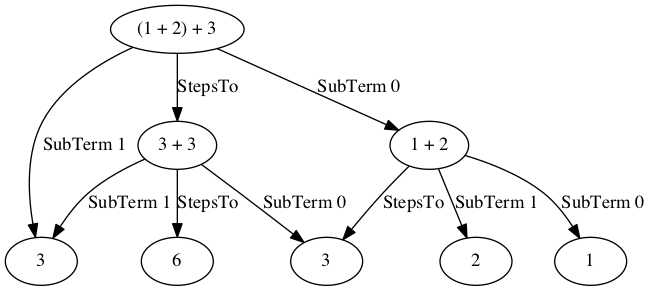
\includegraphics[width=\linewidth]{simple.png}
% \caption{The reduction graph for \texttt{1 + 2 + 3}.}
% \label{fig:simple-reduction}
% \end{figure}
% %
% We choose this graph representation instead of a simple, linear sequence
% of expressions because it will allow us to express a variety of
% traversals, such as ``step into'' and ``step over'' -- commonly found in
% traditional debuggers.



\subsection{Tracing Semantics}
\label{sec:inter-semant}
%
\begin{figure*}[t]
% \relDescription{Trace Syntax}
% $$
% \begin{array}{rrcl}
  % & \tr & ::= & \bullet \spmid \singlestep{e}{e}; \tr \spmid \subterm{e}{e}; \tr
% \end{array}
% $$
% \\
\relDescription{Computing Sub-Terms}
\begin{gather*}
\begin{array}{lcl}
\subtermssym                 & \dcolon & e \to \tr \\
\subterms{\eapp{e_1}{e_2}}   & \defeq & \subterm{\eapp{e_1}{e_2}}{e_1}; \subterm{\eapp{e_1}{e_2}}{e_2} \\
\subterms{\eplus{e_1}{e_2}}   & \defeq & \subterm{\eplus{e_1}{e_2}}{e_1}; \subterm{\eplus{e_1}{e_2}}{e_2} \\
\subterms{\eif{e_1}{e_2}{e_3}}   & \defeq & \subterm{\eif{e_1}{e_2}{e_3}}{e_1}; \\
                                &        & \subterm{\eif{e_1}{e_2}{e_3}}{e_2}; \\
                                &        & \subterm{\eif{e_1}{e_2}{e_3}}{e_3} \\
\subterms{\elet{x}{e_1}{e_2}}   & \defeq & \subterm{\elet{x}{e_1}{e_2}}{e_1}; \\
                                &        & \subterm{\elet{x}{e_1}{e_2}}{e_2} \\
\subterms{\efun{x}{e}}       & \defeq & \subterm{\efun{x}{e}}{e} \\
\subterms{e}                 & \defeq & \bullet
\end{array}
\end{gather*}
\judgementHead{Traced Evaluation}{\stepg{e}{\su}{\tr}{e}{\su}{\tr}}
\begin{gather*}
\inference[\recontext]
  {\stepg{e}{\su}{\tr}{e_1}{\su_1}{\tr_1}}
  {\stepg{C[e]}{\su}{\tr}{C[e_1]}{\su_1}{\singlestep{C[e]}{C[e_1]}; \subterms{C[e_1]}; \tr_1}}
\\ \\
\inference[\reappgood]
  {\pair{\efun{x}{e}}{\su_2} = \force{v_1}{\tfun{\thole{}}{\thole{}}}{\su_1}}
  {\stepg{\eapp{v_1}{v_2}}{\su_1}{\tr}
         {e\sub{x}{v_2}}{\su_1;\su_2}{\singlestep{\eapp{v_1}{v_2}}{e\sub{x}{v_2}}; \subterms{e\sub{x}{v_2}}; \tr}}
\\ \\
\inference[\reappbad]
  {\pair{\stuck}{\su_2} = \force{v_1}{\tfun{\thole{}}{\thole{}}}{\su_1}}
  {\stepg{\eapp{v_1}{v_2}}{\su_1}{\tr}{\stuck}{\su_1;\su_2}{\singlestep{\eapp{v_1}{v_2}}{\stuck}; \tr}}
\end{gather*}
\caption{A selection of the operational semantics from
  Figure~\ref{fig:operational}, extended to collect a full reduction
  graph.}
\label{fig:interactive}
\end{figure*}

\paragraph{Reduction Graphs}
%
A \emph{steps-to} edge is a pair of expressions \singlestep{e_1}{e_2}, which
intuitively indicates that $e_1$ steps, in a single step, to $e_2$.
%
A \emph{sub-term} edge is a pair of expressions \subterm{e_1}{e_2}, which
intuitively indicates that $e_1$ contains $e_2$ as a sub-expression.
%
A \emph{reduction graph} is a set of edges:
$$\tr ::= \bullet \spmid \singlestep{e}{e}; \tr \spmid \subterm{e}{e}; \tr$$

\paragraph{Tracing Semantics}
%
We extend the transition relation (\S~\ref{sec:semantics}) to
collect the set of edges corresponding to the reduction graph.
%
Concretely, we extend the operational semantics to
a relation of the form $\stepg{e}{\vsu}{\tr}{e'}{\vsu'}{\tr'}$
where $\tr'$ collects the edges of the transition.

\paragraph{Collecting Edges}
%
Next, we describe the general recipe for extending a transition
rule to collect edges, and provide a selection of examples
in Figure~\ref{fig:interactive}.
%
The steps-to edges are collected by recording the consequent of
each original rule in the trace. That is, each original judgment
\step{e}{\vsu}{e'}{\vsu'} becomes
\stepg{e}{\vsu}{\tr}{e'}{\vsu'}{\singlestep{e}{e'}; \tr}.
%
The sub-term edges are delegated to a helper function \subtermssym\
which adds edges from an expression to each of its
\emph{immediate} sub-expressions.
%
We collect \subtermssym edges after each transition,
to get the following template for the small-step relation:
\[
\stepg{e}{\vsu}{\tr}{e'}{\vsu'}{\singlestep{e}{e'}; \subterms{e'}; \tr}
\]


% After evaluation the reduction graph can be constructed directly from
% the trace $\tr$ as follows:
% \[
% G(\tr) = \pair{\{e \spmid e \in \tr\}}{\tr}
% \]

% \subsection{Traversing the Reduction Graph}
\subsection{Interactive Debugging}
\label{sec:traversing-graph}

Next, we show how to build an visual interactive debugger
from the traced semantics, by describing the visualization
\emph{state} \ie\ what the user sees at any given moment,
the set of \emph{commands} available to user, and what
they do, and finally how we use a command to \emph{update}
the visualization state. In the sequel, for clarity of
exposition, we assume we have a (global) trace:
$\stepg{e}{\emptysu}{\bullet}{e'}{\vsu'}{\tr}$.

\paragraph{State}
A \emph{visualization state} is ...
The \emph{initial state} is the graph containing the single edge
${e \hookrightarrow \stuck}$.
+ Visualization = ExprGraph + invariants (unique predecessor) -- link to figure.

\paragraph{Commands}
\begin{itemize}
\item \stepforwardsym\ takes a single step forward.
\item \stepbackwardsym\ takes a single step backward.
\item \jumpforwardsym\ takes a ``big'' step forward to the next function call.
\item \jumpbackwardsym\ takes a ``big'' step backward to the previous function call.
\item \stepintosym\ steps into a function call in a sub-term, isolating it from the context.
\item \stepoversym\ steps over a function call in a sub-term.
\end{itemize}

\paragraph{Update}
Figure~\ref{fig:traversing-graph} shows how we update the state for each
command...
%
find   :: Vis -> Cmd -> Expr
update :: Vis -> Cmd -> Vis
%
The initial path $p$ is required for the backward-steps as a node may
have multiple incoming $\leadsto$ edges, \eg
\singlestep{\eplus{1}{2}}{3} and \singlestep{\eplus{2}{1}}{3}.
%
Note that the sub-term edges $\searrow$ allow us to decompose an expression into a
sub-expression and the surrounding context, thus enabling the \stepintosym
and \stepoversym traversals.



data Sel = Expr

data Vis = { graph :: TraceGraph, edges = ExprGraph  }

path :: Vis -> Expr -> [Expr]
stepX :: Sel -> Vis -> Vis(edited)

path v e = graphPath (graph v,  root (v, e),  e)

putBefore, putAfter :: EGraph -> Expr -> Expr -> EGraph
putRoot  :: EGraph -> Expr -> EGraph
getRoot  :: EGraph -> Expr -> Expr

pathToRoot  ::


\begin{figure*}[t]
\centering
\[
\begin{array}{lcl}
\stepforward{G}{p}{e_i}  &\defeq& \left\{\begin{array}{ll}
    e_j, & \text{where } \singlestep{e_i}{e_j} \in G
                         \end{array}\right\} \\ \\
\stepbackward{G}{p}{e_i}  &\defeq& \left\{\begin{array}{ll}
    e_j, & \text{where } \singlestep{e_j}{e_i} \in G \text{ and } e_j \in p
                         \end{array}\right\} \\ \\
\jumpforward{G}{p}{e_i} &\defeq& \text{let } e_j = \stepforward{G}{p}{e_i} \text{ in }
                         \left\{\begin{array}{ll}
                         e_j, & \text{if } e_j = \eapp{v_1}{v_2} \\
                         \jumpforward{G}{p}{e_{j}}, & \text{otherwise}
                         \end{array}\right\} \\ \\
\jumpbackward{G}{p}{e_i} &\defeq& \text{let } e_j = \stepbackward{G}{p}{e_i} \text{ in }
                         \left\{\begin{array}{ll}
                         e_j, & \text{if } e_j = \eapp{v_1}{v_2} \\
                         \jumpbackward{G}{p}{e_{j}}, & \text{otherwise}
                         \end{array}\right\} \\ \\
\stepinto{G}{p}{e_i} &\defeq& \left\{\begin{array}{ll}
                         e\sub{x}{v_2}, & \text{if } e_i = C[\eapp{v_1}{v_2}] \text{ and } \singlestep{\eapp{v_1}{v_2}}{e\sub{x}{v_2}}
                         \end{array}\right\} \\ \\
\stepover{G}{p}{e_i} &\defeq& \left\{\begin{array}{ll}
                         C[v], & \text{if } e_i = C[\eapp{v_1}{v_2}] \text{ and } \multistep{\eapp{v_1}{v_2}}{v}
                         \end{array}\right\}
\end{array}
\]
\caption{Rules for traversing the reduction graph given a path and
  node. \stepintosym and \stepoversym require a traversal of the
  sub-term edges to decompose $e_i$ into the target expression
  \eapp{v_1}{v_2} and the context $C$.  \ES{these rules are quite ugly and waste space..} }
\label{fig:traversing-graph}
\end{figure*}
